\newchapstyle
\chapter{Probing the current-phase relation of graphene Josephson junctions
with microwave circuits}
\label{chap:gJJ-CPR}


\begin{abstract}
	Smart sounding abstract
\end{abstract}

%% Start the actual chapter on a new page.
\newpage

\begin{align}
f_0(I_b,I_c) = \frac{f_r}{1 +  \frac{L_j(I_b, I_c)}{L_r}}
\end{align}

\begin{align}
L_J = \frac{\Phi_0}{2\pi}\left(\diff{I_s}{\delta}\right)^{-1} = \frac{\Phi_0}{2\pi\sqrt{I_c^2-I_b^2}}
\end{align}

\begin{align}
I_s(\delta,\tau,T) = \frac{\pi\Delta}{2 e R_n} \frac{\sin\delta}{\sqrt{1 - \tau \sin^2\delta / 2}} \tanh\left(\frac{\Delta}{k_B T} \sqrt{1 - \tau \sin^2\delta / 2}\right)
\end{align}

$I_c(\tau,T)=\underaccent{\delta}{\max} \left[I_s(\delta,\tau,T)\right]$

$R_n= h/(Ne^2)\approx \SI{25.812}{\kilo\ohm} / N$.
%
With a normal state resistance ranging between \SIrange{35}{350}{\ohm} (depending on gate voltage), we estimate around 74 to 740 conducting channels.

\begin{align}
\alpha=-\frac{\omega_0}{2} \left(\frac{L_J}{L_r+L_J}\right)^3 = E_C \left( 1-\frac{3}{4}\frac{\sum_i\tau_i^2}{\sum_i\tau_i}\right) \approx E_C \left( 1-\frac{3}{4}\tau \right)
\end{align}
\cite{Zhou,Microsoft}





\begin{figure}
	\centering
	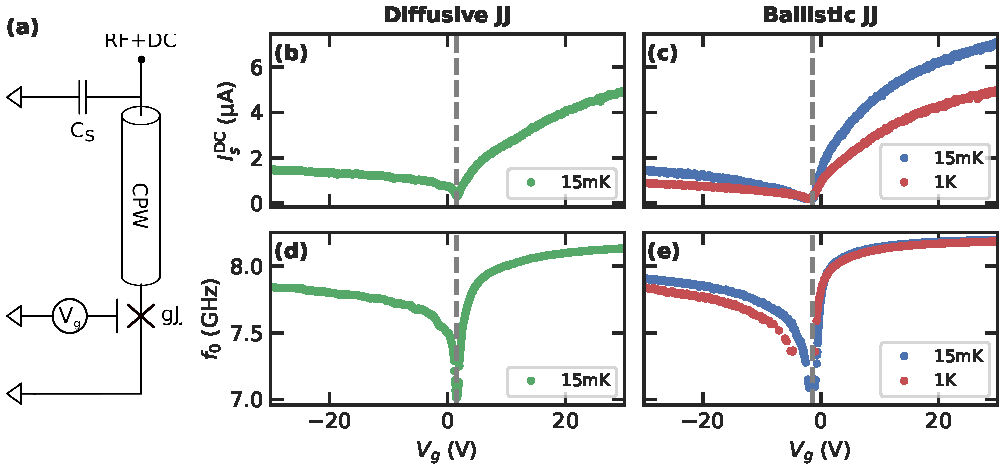
\includegraphics[width=\linewidth]{chapter-gJJ-CPR/figs/Figure1}
	\caption{
	\textbf{A graphene Josephson junction embedded in a DC bias microwave circuit.}
	\textbf{(a)} Measurement schematic.
	The gJJ shorts a coplanar waveguide transmission line to ground, which
forms a gate-tunable $\lambda/2$-resonator.
	\textbf{(b-e)} Switching currents (top row) for the diffusive \textbf{(b)} and ballistic Josephson junction \textbf{(d)}, at base-temperature of \SI{15}{\milli\kelvin} (blue) and at \SI{1}{\kelvin} (red).
	Bottom row: Resonance frequencies versus gate voltage for the diffusive \textbf{(c)} and ballistic \textbf{(e)} device.
	The gate-tunable Josephson inductance changes the
boundary condition of the $\lambda/2$-resonator, thus changing the resonance frequency of the circuit.}
	\label{fig:figure1}
\end{figure}

\begin{figure}
	\centering
	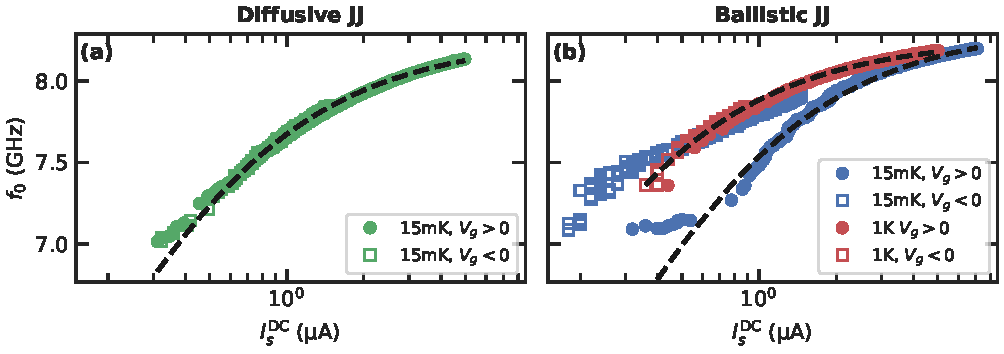
\includegraphics[width=0.5\linewidth]{chapter-gJJ-CPR/figs/Figure2}
	\caption{
	\textbf{Resonance frequency vs switching currents for two different gJJ devices.}
	Both the diffusive device at low temperature \textbf{(a)} and the ballistic device at \SI{1}{\kelvin} (\textbf{(b)}, red) show monotonically increasing $f_0$ versus DC-extracted switching currents.
	In contrast, for low temperatures, the ballistic gJJ (\textbf{(b)}, blue) exhibits multi-valued $f_0(I_s)$ for gate voltages larger (full circles) and smaller (empty squares) than the charge neutrality point.
	The	multivalued behavior in the ballistic device at low temperature indicates a strong
nonsinusoidal CPR, while this is not observed for diffusive and hot
transport.
	Dashed lines correspond to fits to Eq.~\ref{eq:Pogorzalek}.}
	\label{fig:figure2}
\end{figure}
\begin{figure}
	\centering
	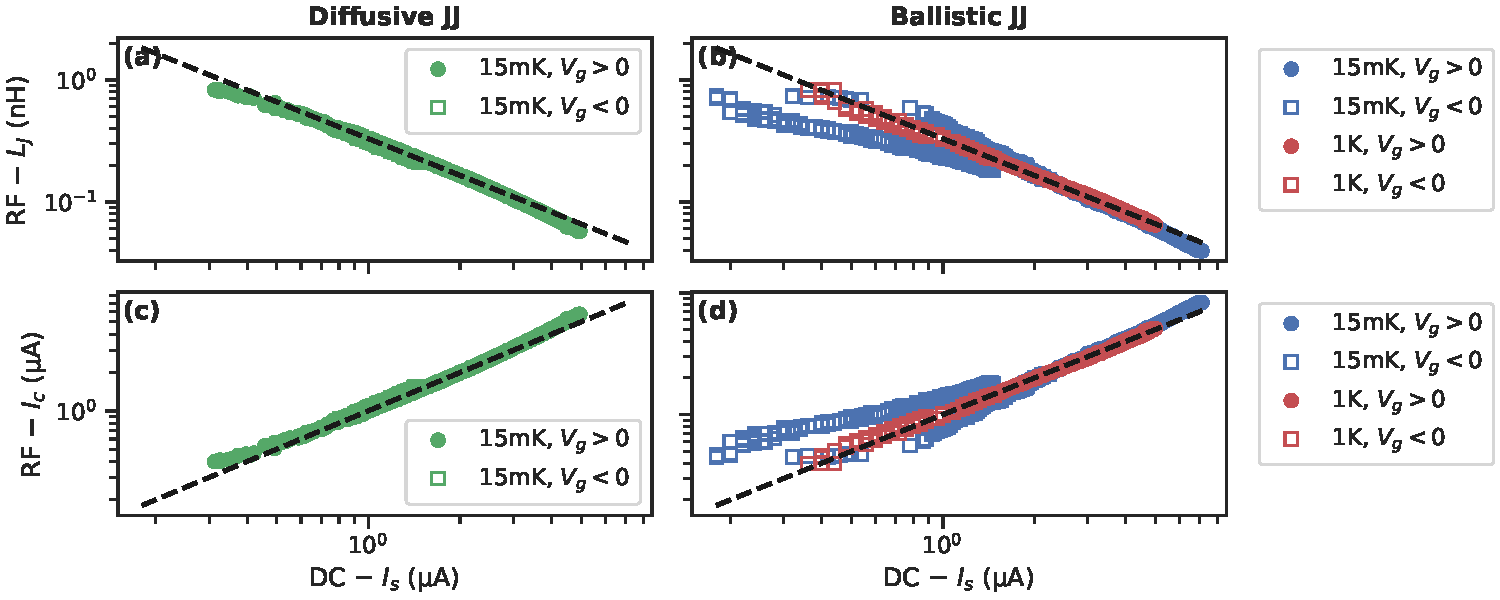
\includegraphics[width=0.833\linewidth]{chapter-gJJ-CPR/figs/Figure3}
	\caption{
	\textbf{Comparing switching current and Josephson inductance.}
	Both scattering in the JJ as well as elevated temperatures reduce the deviation from RF and DC data.
	\textbf{(a-b)} RF-extracted Josephson inductance versus DC-measured switching current for the diffusive device at
	\SI{15}{\milli\kelvin} \textbf{(a)} and ballistic device at \SI{15}{\milli\kelvin} and at \SI{1}{\kelvin} (\textbf{(b)}, blue and red, respectively).
	Solid line corresponds to Josephson inductance
calculated from sinusoidal CPR.
	\textbf{(c-d)} Corresponding RF-extracted critical current.
	Solid line corresponds to DC-measured $I_s$.}
	\label{fig:figure3}
\end{figure}
\begin{figure}
	\centering
	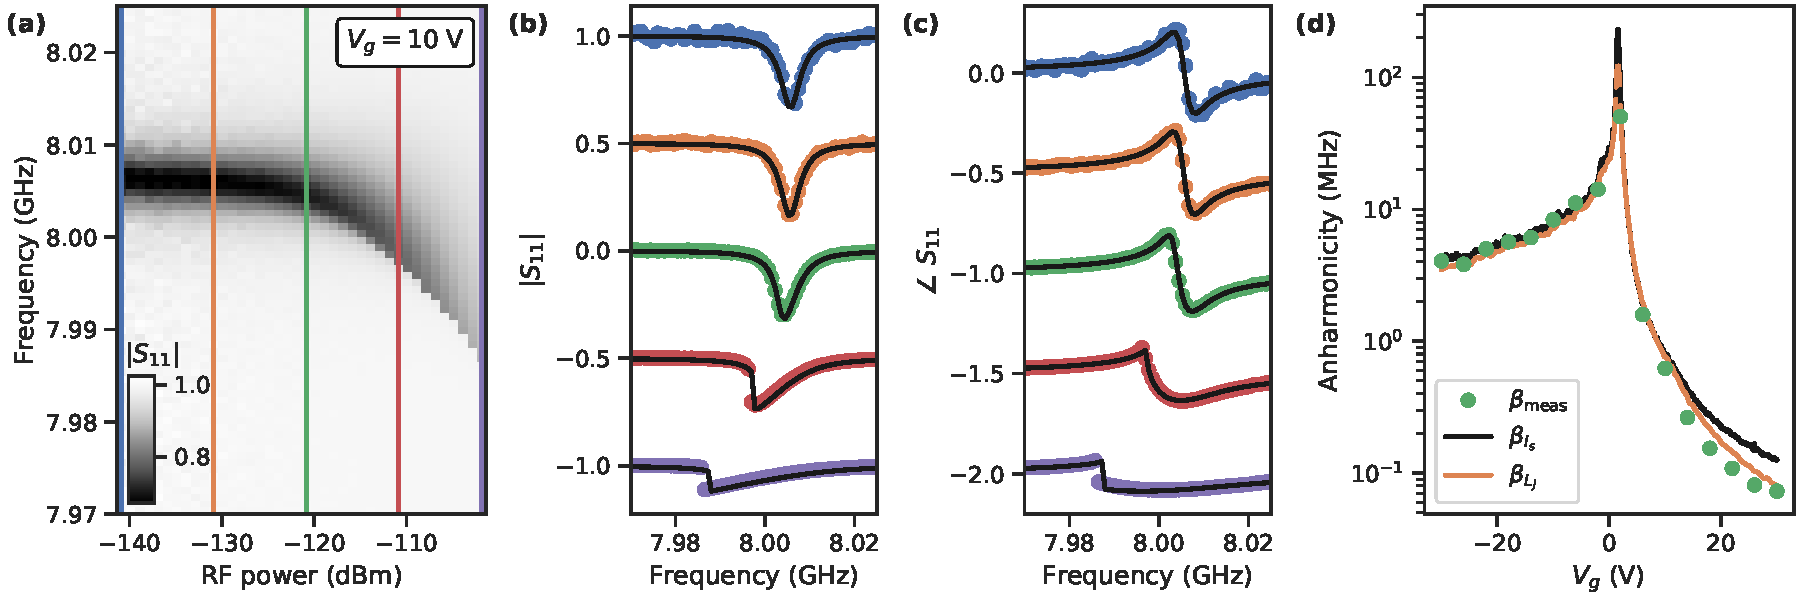
\includegraphics[width=\linewidth]{chapter-gJJ-CPR/figs/Figure4}
	\caption{
	\textbf{Power dependence of a nonlinear microwave device with diffusive gJJ.}
	\textbf{(a)} Absolute value of the reflection coefficient $S_{11}$ versus frequency for increasing drive power.
	Due to the Kerr
nonlinearity, the resonator experiences a downshift and bifurcation at elevated drive powers.
	Solid
lines indicate linecuts in \textbf{(b)} and \textbf{(c)}.
	\textbf{(b-c)} Absolute value \textbf{(b)} and phase \textbf{(c)} of $S_{11}$ for varying drive power as indicated in \textbf{(a)}.
	Black lines
are fits.
	\textbf{(d)} Anharmonicity vs gate voltage.
	Dots: data as extracted from fits as in \textbf{(b-c)}, orange line: model
using DC-$I_s$, green: model using RF-$I_c$.
	The overestimation of the anharmonicity of the DC-$I_s$ for high
gate voltages hints at a non-sinusoidal CPR.}
	\label{fig:figure4}
\end{figure}
\begin{figure}
	\centering
	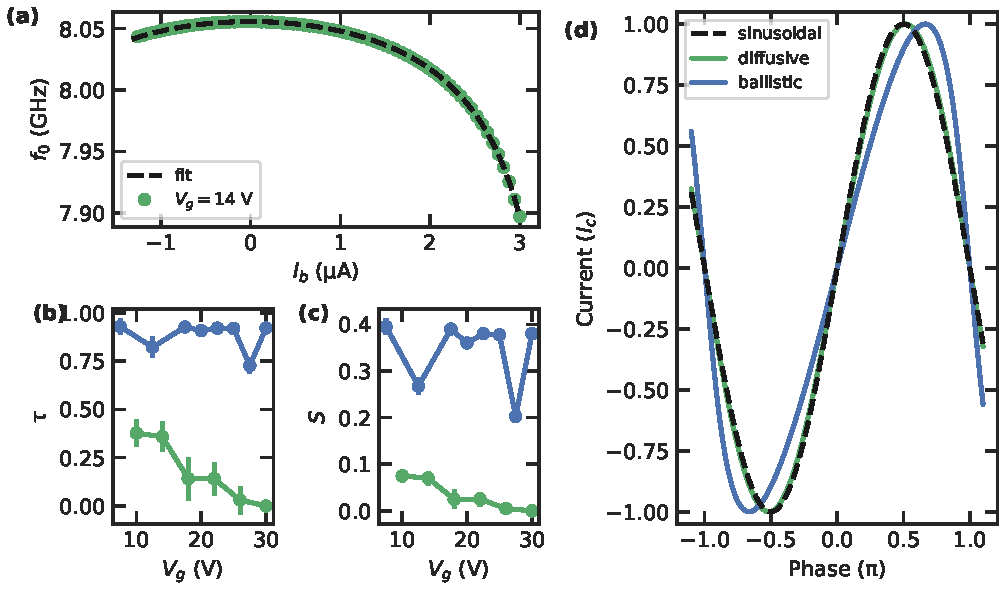
\includegraphics[width=\linewidth]{chapter-gJJ-CPR/figs/Figure5}
	\caption{
	\textbf{Influence of the junction transparency on the bias current dependence.}
	\textbf{(a)} CPR for various $\tau=0$ (solid), $\tau=0.5$ (dashed) and $\tau=1.0$	(dash-dotted).
	\textbf{(b-c)} Josephson inductance \textbf{(b)} and resonance frequency \textbf{(c)} supercurrent for	same transparencies as in \textbf{(a)}.
	Increased junction transmission leads to forward skewing of the CPR, thus a
reduced slope and higher Josephson inductance, which in turn reduces the
resonance frequency and increases the tuning.}
	\label{fig:figure5}
\end{figure}
\begin{figure}
	\centering
	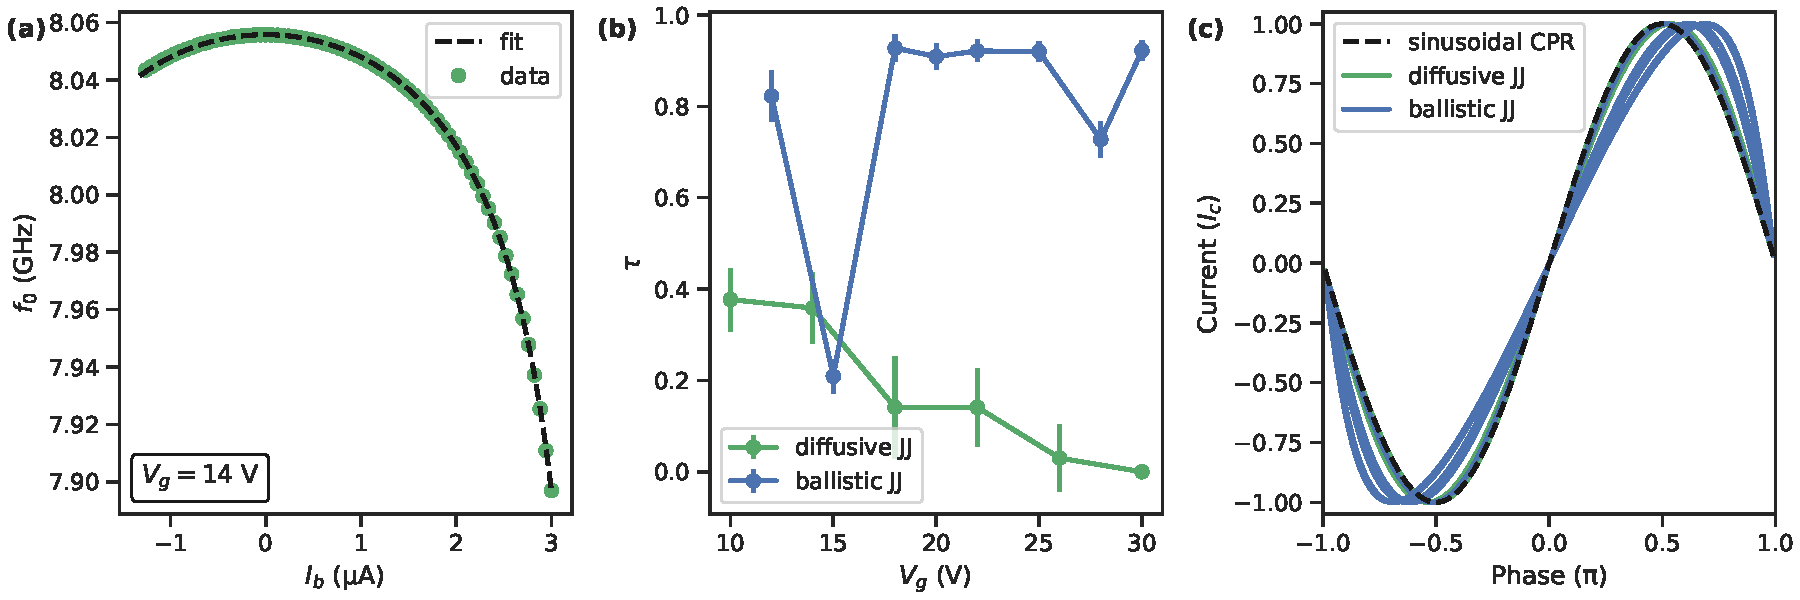
\includegraphics[width=\linewidth]{chapter-gJJ-CPR/figs/Figure6}
	\caption{
	\textbf{Extracting the current phase relation from current-biasing the gJJ microwave circuit.}
	Fitting the bias current dependence \textbf{(a)}, we can extract the junction transparency \textbf{(b)} for the diffusive (green) and ballistic
(blue) gJJ device versus gate voltage.
	\textbf{(c)} Reconstructed current-phase relation for the diffusive (green) and ballistic (blue) device.
	The large transparency of the ballistic JJ leads to significant forward skewing, while the relatively low
transparency of the diffusive JJ only results in minor skewing.}
	\label{fig:figure6}
\end{figure}

\references{dissertation}

